% Date : 06/03/2023
% Version : 3
% Auteur : SBA
% Relu : oui
% Relecteur : JRL, CBD,  Florence Gouttverg
% Harmonisateur: GBU
% Version harmonisation: 3

% ------------------------------------------------------------ %
% ----------------------  Fiche MAG02  ----------------------- %
% Thème : particules dans un champ EM
% Classes : MPSI-PCSI-PTSI-MP2I
% ------------------------------------------------------------ %



% ======================================================= % 
% ============== Gestion de la compilation ============== %
% ======================================================= % 
\ifdefined\mainIsLoaded\else
\RequirePackage{import}
\subimport{../../}{_preambule_CdE_PC}
\begin{document}
\fi
% ======================================================= % 
% ======================================================= % 



% ======================================================= % 
% ===================== Couleurs ======================== %
% ======================================================= % 

% -----------------------------------%
% La commande \couleurNBouCouleur prend deux paramètres :
% #1 est la couleur NB ; #2 est la couleur "en couleur"
\def\JRLblue{\couleurNBouCouleur{black}{blue!75}}
 \def\JRLblueC{\couleurNBouCouleur{lightgray!30}{blue!15}}
 \def\JRLblueF{\couleurNBouCouleur{darkgray}{blue!50}}
\def\JRLred{\couleurNBouCouleur{darkgray}{red!66}}
 \def\JRLcyan{\couleurNBouCouleur{gray}{cyan}}
 \def\JRLcyanclair{\couleurNBouCouleur{lightgray!30}{cyan!10}}
% ======================================================= % 




% ============================================================================ %
%                            FICHE D'ENTRAÎNEMENT                              %
% ============================================================================ %
% ======================= Métadonnées sur la fiche =========================== %
\titreFicheEntrainement		{Particule dans un champ électromagnétique}
\grandTheme					{Électromagnétisme}
\numeroFiche				{MAG02}
\uniqueID					{yanVCxMUOZP} % une chaîne de caractères (a-z, A-Z) aléatoire de 10 caractères.
\nombreColonnesReponses		{3} % 1, 2, 3, etc.
% ============================================================================ %

%%%%%%%%%%%%%%%%%%%%%%%%%%%%%%%%%%%%%%%%%%%%%%%%%%%%%%%%%%%%%%%%%%%%%%%%%%%%%%%%%%%%%%%%%%%%%%
\debutFicheEntrainement                                                                      %
%%%%%%%%%%%%%%%%%%%%%%%%%%%%%%%%%%%%%%%%%%%%%%%%%%%%%%%%%%%%%%%%%%%%%%%%%%%%%%%%%%%%%%%%%%%%%%



% --------------------------------------------------------------------- %
%                              Prérequis                                %
%                             (facultatif)                              %
% --------------------------------------------------------------------- %
% ================== Métadonnées sur le prérequis ===================== %
\avecPrerequis{Y} % Y ou N
% ===================================================================== %
\begin{prerequis}
Principe fondamental de la dynamique. Théorème de l'énergie cinétique, 
de l'énergie mécanique. Puissance, travail. Énergie potentielle. \\Force de Lorentz.

\constantesUtiles
	\begin{listeConstantes}
		\item charge élémentaire : $e=\SI{1.60e-19}{C}$
		\item célérité de la lumière dans le vide : $c=\SI{3.00e8}{m.s^{-1}}$
	\end{listeConstantes}

\end{prerequis}
% --------------------------------------------------------------------- %






% •••••••••••••••••••••••••••••••••••••••••••••••••••••••••••••••••••••••••••• %
% •••••••••••••••••••••••••••••••••••••••••••••••••••••••••••••••••••••••••••• %
\sectionFicheEntrainement{Préliminaires}
% •••••••••••••••••••••••••••••••••••••••••••••••••••••••••••••••••••••••••••• %
% •••••••••••••••••••••••••••••••••••••••••••••••••••••••••••••••••••••••••••• %



% ********************************************************************* %
%                           ENTRAÎNEMENT                                % 
% ********************************************************************* %
% ================ Métadonnées sur l'entraînement ===================== %
\titreEntrainementFacultatif	{Électron-volt}
\hauteurLargeurCadreReponse		{7mm}{3cm}
\dureeResolutionFacultative		{2} % 1, 2, 3 ou 4
\typeEntrainement				{AN} % Newton ou QCM ou AN ou vide (exercice "normal")
\nombreColonnesQuestions		{1} % vide, 1, 2, 3, etc.
\avecPlusieursQuestions			{Y} % Y ou N
\initialisationEntrainement
% ===================================================================== %

Le produit d'une charge électrique par une tension est une énergie. 

En multipliant la charge élémentaire $e=\SI{1.6e-19}{\coulomb}$ par une tension de \SI{1}{\volt}, on obtient une unité adaptée à la physique des particules, l'électron-volt, noté $\si{eV}$.
On a $\SI{1}{eV} = \SI{1.6e-19}{J}$. 

% =============================================================================== %
\debutEntrainement
% =============================================================================== %

% ^^^^^^^^^^^^^^^^^^^^^^^^^^^^^^^^^^^^^^ %
%               Question                 %
% ^^^^^^^^^^^^^^^^^^^^^^^^^^^^^^^^^^^^^^ %

\begin{enonce}
Que vaut \SI{1}{J} en \si{eV}?
\end{enonce}

\reponse{\SI{6.3e18}{eV}}

\begin{corrige}
On a $\SI{1}{eV} = \SI{1,6e-19}{J}$, $\SI{1}{J}= 1/\num{1,6e-19} \si{eV} = \SI{6,3e18}{eV}$.
\end{corrige}

% ************************************** %

% ^^^^^^^^^^^^^^^^^^^^^^^^^^^^^^^^^^^^^^ %
%               Question                 %
% ^^^^^^^^^^^^^^^^^^^^^^^^^^^^^^^^^^^^^^ %

\begin{enonce}
L'énergie d'un photon rouge est de \SI{2,48e-19}{J}. \minusMedskip\\ Convertir en \si{eV}.
\end{enonce}

\reponse{\SI{1,55}{eV}}

\begin{corrige}
On a $\SI{2,48e-19}{J} = \SI{2,48e-19}{J} \times \SI{6,3e18}{eV/J} = \SI{1,55}{eV}$.
\end{corrige}

% ************************************** %

% ^^^^^^^^^^^^^^^^^^^^^^^^^^^^^^^^^^^^^^ %
%               Question                 %
% ^^^^^^^^^^^^^^^^^^^^^^^^^^^^^^^^^^^^^^ %

\begin{enonce}
L'énergie d'un photon violet est de $\SI{3,1}{eV}$. \minusMedskip\\ Convertir en \si{J}.
\end{enonce}

\reponse{\SI{5,0e-19}{J}}

\begin{corrige}
On a $\SI{3,1}{eV} =\SI{3,1}{eV}\times \SI{1,6e-19}{J/eV} = \SI{5,0e-19}{J}$.
\end{corrige}

% ************************************** %

% ^^^^^^^^^^^^^^^^^^^^^^^^^^^^^^^^^^^^^^ %
%               Question                 %
% ^^^^^^^^^^^^^^^^^^^^^^^^^^^^^^^^^^^^^^ %

\begin{enonce}
Quel photon a la plus grande énergie ? \minusMedskip\\Le rouge ou le violet ?
\end{enonce}

\reponse{violet}

\begin{corrige}
On peut comparer les énergies en eV: $E_\text{violet} = \SI{3,1}{eV} > \SI{1,55}{eV} =E_\text{rouge}$. 
\end{corrige}

% ************************************** %

% =============================================================================== %
\finEntrainement
% =============================================================================== %




% ********************************************************************* %
%                           ENTRAÎNEMENT                                % 
% ********************************************************************* %
% ================ Métadonnées sur l'entraînement ===================== %

\pointInterrogation				{Y}
\titreEntrainementFacultatif	{Qui est le plus massique}
\hauteurLargeurCadreReponse		{8mm}{3cm}
\dureeResolutionFacultative		{1} % 1, 2, 3 ou 4
\typeEntrainement				{Newton} % Newton ou QCM ou AN ou vide (exercice "normal")
\nombreColonnesQuestions		{1} % vide, 1, 2, 3, etc.
\avecPlusieursQuestions			{N} % Y ou N
\initialisationEntrainement
% ===================================================================== %


% =============================================================================== %
\debutEntrainement
% =============================================================================== %

On considère les trois particules suivantes :
\begin{itemize}
\item le proton, dont la masse vaut $m_{\text{proton}}=\SI{1.67e-27}{kg}$ ;

\item le {kaon}, qui est une particule
dont l'énergie de masse vaut $m_{\text{kaon}} \times c^{2}=\SI{7.90e-4}{erg}$ ;

\item le {tau}, qui est une particule 
de masse $m_{\text{tau}} = \SI{1777}{MeV/c^{2}}$.
\end{itemize}
\smallskip

On donne $\SI{1}{erg}=\SI{1}{g.cm^{2}.s^{-2}}$ et $\SI{1}{eV} = \SI{1.6e-19}{J}$.

% ^^^^^^^^^^^^^^^^^^^^^^^^^^^^^^^^^^^^^^ %
%               Question                 %
% ^^^^^^^^^^^^^^^^^^^^^^^^^^^^^^^^^^^^^^ %


\begin{enonce}
Laquelle de ces particules est la plus massique ?
\end{enonce}

\reponse{tau}

\begin{corrige}
On a $\SI{1}{erg}=\SI{1}{g.cm^{2}.s^{-2}}=10^{-3}\times\left(10^{-2}\right)^{2}\si{kg.m^{2}.s^{-2}}=\SI{1e-7}{J}$.

Avec $c=\SI{3.00e8}{m.s^{-1}}$, la masse de kaon peut s'écrire en
$\si{kg}$:
\[
m_{\text{kaon}}=\dfrac{\SI{7.90e-11}{J}}{\left(\SI{3.00e8}{m.s^{-1}}\right)^{2}}=\SI{8.78e-28}{kg}.
\]
Comme $\SI{1}{eV} = \SI{1.6e-19}{J}$, on a
\[
m_{\text{tau}}=\dfrac{\num{1777e6}\times\SI{1.6e-19}{J}}{\left(\SI{3.00e8}{m.s^{-1}}\right)^{2}}=\SI{3.16e-27}{kg}.
\]
C'est donc la particule tau la plus massique.
\end{corrige}

% ************************************** %

%================================================================================ %
\finEntrainement
% =============================================================================== %








\newpage


% •••••••••••••••••••••••••••••••••••••••••••••••••••••••••••••••••••••••••••• %
% •••••••••••••••••••••••••••••••••••••••••••••••••••••••••••••••••••••••••••• %
\sectionFicheEntrainement{Champ électrique et potentiel scalaire}
% •••••••••••••••••••••••••••••••••••••••••••••••••••••••••••••••••••••••••••• %
% •••••••••••••••••••••••••••••••••••••••••••••••••••••••••••••••••••••••••••• %



% ********************************************************************* %
%                           ENTRAÎNEMENT                                % 
% ********************************************************************* %
% ================ Métadonnées sur l'entraînement ===================== %

\pointInterrogation				{N}
\titreEntrainementFacultatif	{Carte d'équipotentielles}
\hauteurLargeurCadreReponse		{8mm}{3.5cm}
\dureeResolutionFacultative		{1} % 1, 2, 3 ou 4
\typeEntrainement				{Newton} % Newton ou QCM ou AN ou vide (exercice "normal")
\nombreColonnesQuestions		{1} % vide, 1, 2, 3, etc.
\avecPlusieursQuestions			{Y} % Y ou N
\initialisationEntrainement
% ===================================================================== %



% =============================================================================== %
\debutEntrainement
% =============================================================================== %
On représente ci-dessous la carte des équipotentielles créées par trois
charges électriques. 

Une équipotentielle correspond à l'ensemble des
lieux où le potentiel électrostatique scalaire $V$ prend une même
valeur numérique.

\begin{center}
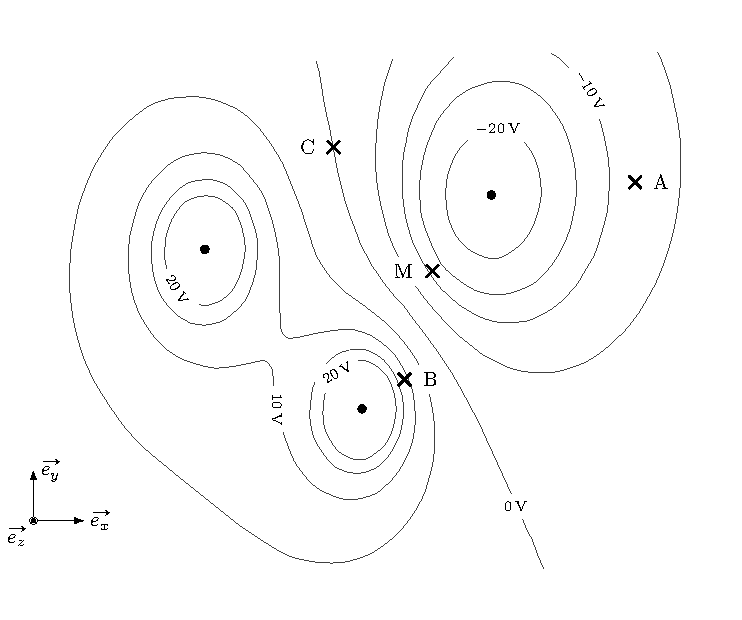
\includegraphics{_images/fiche_MAG02_equipotentielles_for_PDF.pdf}
\end{center}


% ^^^^^^^^^^^^^^^^^^^^^^^^^^^^^^^^^^^^^^ %
%               Question                 %
% ^^^^^^^^^^^^^^^^^^^^^^^^^^^^^^^^^^^^^^ %

\begin{enonce}
En norme, le champ électrique est le plus intense:
\begin{listeQCM3Colonnes}
\item en \ptA %$\,$
\item en \ptB %$\,$
\item en \ptC %$\,$
\end{listeQCM3Colonnes}
\bigskip
\end{enonce}

\reponse{\reponseB{}}

\begin{corrige}
Le champ est d'autant plus intense en norme que les équipotentielles sont proches: pour un même déplacement $\vv{\d{}\ell}$ la variation du potentiel électrique est plus importante.
\end{corrige}

% ************************************** %

% ^^^^^^^^^^^^^^^^^^^^^^^^^^^^^^^^^^^^^^ %
%               Question                 %
% ^^^^^^^^^^^^^^^^^^^^^^^^^^^^^^^^^^^^^^ %

\begin{enonce}
En M, le champ électrique est orienté :
 \begin{listeQCM2Colonnes}
\item vers en haut à droite
\item vers en haut à gauche
\item vers en bas à droite
\item vers en bas à gauche
\end{listeQCM2Colonnes}

% ************************************** %

% ^^^^^^^^^^^^^^^^^^^^^^^^^^^^^^^^^^^^^^ %
%               Question                 %
% ^^^^^^^^^^^^^^^^^^^^^^^^^^^^^^^^^^^^^^ %

\end{enonce}
\reponse{\reponseA{}}%
\begin{corrige}
Le champ électrique est orienté dans le sens des
potentiels décroissants et orthogonal aux équipotentielles. Le champ est donc orienté vers le haut à droite.
\end{corrige}

% ************************************** %

%================================================================================ %
\finEntrainement
% =============================================================================== %



\newpage


% ********************************************************************* %
%                           ENTRAÎNEMENT                                % 
% ********************************************************************* %
% ================ Métadonnées sur l'entraînement ===================== %

\pointInterrogation				{N}
\titreEntrainementFacultatif	{Potentiel scalaire}
\hauteurLargeurCadreReponse		{8mm}{2.5cm}
\dureeResolutionFacultative		{2} % 1, 2, 3 ou 4
\typeEntrainement				{Newton} % Newton ou QCM ou AN ou vide (exercice "normal")
\nombreColonnesQuestions		{2} % vide, 1, 2, 3, etc.
\avecPlusieursQuestions			{Y} % Y ou N
\initialisationEntrainement
% ===================================================================== %


Le potentiel électrostatique scalaire $V$ vérifie 
\[
\d{}V\left(\ptM\right)=-\vv{E}\left(\ptM\right)\cdot\vv{\d{}\ell}
\]
 où $\vv{\d{}\ell}$ est le vecteur déplacement
élémentaire.

On rappelle les expressions du vecteur $\vv{\d{}\ell}$
en coordonnées cartésiennes 
et en coordonnées cylindriques : 
\begin{align*}
\vv{\d{}\ell} & =\d{}x\vv{e_{x}}+\d{}y\vv{e_{y}}+\d{}z\vv{e_{z}} \\
           & =\d{}r\vv{e_{r}}+r\d{}\theta\vv{e_{\theta}}+\d{}z\vv{e_{z}}.
\end{align*}

En déterminant $\d{}V$, puis intégrant, exprimer le potentiel $V(\ptM)$ pour les champs $\vv{E}$ suivants : 

% =============================================================================== %
\debutEntrainement
% =============================================================================== %


% ^^^^^^^^^^^^^^^^^^^^^^^^^^^^^^^^^^^^^^ %
%               Question                 %
% ^^^^^^^^^^^^^^^^^^^^^^^^^^^^^^^^^^^^^^ %

\begin{enonce}
$\vv{E}(\ptM)=E\vv{e_{x}}$ 
\end{enonce}

\reponse{$-Ex+C$}

\begin{corrige}
En effet, on commence par trouver $\d{}V\left(\ptM\right)=-E\d{}x=\d{}\left(-Ex+C\right)$.
\end{corrige}

% ************************************** %

% ^^^^^^^^^^^^^^^^^^^^^^^^^^^^^^^^^^^^^^ %
%               Question                 %
% ^^^^^^^^^^^^^^^^^^^^^^^^^^^^^^^^^^^^^^ %

\begin{enonce}
$\vv{E}(\ptM)=\dfrac{\alpha}{r^{2}}\vv{e_{r}}$
\end{enonce}
\reponse{$\dfrac{\alpha}{r}+C$}%
\begin{corrige}
En effet, on commence par trouver $\d{}V\left(\ptM\right)=-\alpha\dfrac{\d{}r}{r^{2}}=\d{}\left(\dfrac{\alpha}{r}+C\right)$.
\end{corrige}

% ************************************** %

% ^^^^^^^^^^^^^^^^^^^^^^^^^^^^^^^^^^^^^^ %
%               Question                 %
% ^^^^^^^^^^^^^^^^^^^^^^^^^^^^^^^^^^^^^^ %

\begin{enonce}
$\vv{E}\left(\ptM\right)=\dfrac{\beta}{r}\vv{e_{r}}$
\end{enonce}

\reponse{$-\beta\ln(r)+C$}

\begin{corrige}
En effet, on commence par trouver $\d{}V\left(\ptM\right)=-\beta\dfrac{\d{}r}{r}=\d{}\left(-\beta\ln(r)+C\right)$.
\end{corrige}

% ************************************** %

% ^^^^^^^^^^^^^^^^^^^^^^^^^^^^^^^^^^^^^^ %
%               Question                 %
% ^^^^^^^^^^^^^^^^^^^^^^^^^^^^^^^^^^^^^^ %

\begin{enonce}
$\vv{E}\left(\ptM\right)=\gamma\left(y\vv{e_{x}}+x\vv{e_{y}}\right)$
\end{enonce}

\reponse{$-\gamma xy+C$}

\begin{corrige}
En effet, on commence par trouver $\d{}V\left(\ptM\right)=-\gamma\left(y\d{}x+x\d{}y\right)=\d{}\left(-\gamma xy+C\right)$.
\end{corrige}

% ************************************** %

%================================================================================ %
\finEntrainement
% =============================================================================== %















% •••••••••••••••••••••••••••••••••••••••••••••••••••••••••••••••••••••••••••• %
% •••••••••••••••••••••••••••••••••••••••••••••••••••••••••••••••••••••••••••• %
\sectionFicheEntrainement{Force de Lorentz}
% •••••••••••••••••••••••••••••••••••••••••••••••••••••••••••••••••••••••••••• %
% •••••••••••••••••••••••••••••••••••••••••••••••••••••••••••••••••••••••••••• %

\bigskip

On rappelle l'expression de la force de Lorentz $\vv{F_L}=q(\vv{E}+\vv{v}\wedge \vv{B})$.



% ********************************************************************* %
%                           ENTRAÎNEMENT                                % 
% ********************************************************************* %
% ================ Métadonnées sur l'entraînement ===================== %

\pointInterrogation				{N}
\titreEntrainementFacultatif	{Composante électrique de la force de Lorentz}
\hauteurLargeurCadreReponse		{8mm}{5cm}
\dureeResolutionFacultative		{1} % 1, 2, 3 ou 4
\typeEntrainement				{Newton} % Newton ou QCM ou AN ou vide (exercice "normal")
\nombreColonnesQuestions		{1} % vide, 1, 2, 3, etc.
\avecPlusieursQuestions			{Y} % Y ou N
\initialisationEntrainement
% ===================================================================== %



Dans la base $\left(\vv{e_{x}},\vv{e_{y}},\vv{e_{z}}\right)$,
exprimer (en fonction de $q$, de $E$ et éventuellement de $\alpha$ et $\beta$) la composante électrique de la force de Lorentz, définie par $\vv{F}_{L,\text{électrique}}=q\vv{E}$.


\begin{center}
\subimport{_images/}{fiche_MAG02_chpE_F_electrique_CBD_v2.tex}
\end{center}


\minusBigskip

% =============================================================================== %
\debutEntrainement
% =============================================================================== %

% ^^^^^^^^^^^^^^^^^^^^^^^^^^^^^^^^^^^^^^ %
%               Question                 %
% ^^^^^^^^^^^^^^^^^^^^^^^^^^^^^^^^^^^^^^ %

\begin{enonce}
$\vv{F}_{L,\text{électrique}}=$
\end{enonce}

\reponse{$qE\vv{e_{y}}$}

\begin{corrige}
La force est indépendante de la vitesse. On trouve
$\vv{F}_{L,\text{électrique}}=q\vv{E}=qE\vv{e_{y}}$.
\end{corrige}

% ************************************** %

% ^^^^^^^^^^^^^^^^^^^^^^^^^^^^^^^^^^^^^^ %
%               Question                 %
% ^^^^^^^^^^^^^^^^^^^^^^^^^^^^^^^^^^^^^^ %

\begin{enonce}
$\vv{F}_{L,\text{électrique}}=$
\end{enonce}

\reponse{$\va{qE}\vv{e_{x}}$}

\begin{corrige}
On trouve $\vv{F}_{L,\text{électrique}}=q\vv{E}=\va{qE}\vv{e_{x}}$.
\end{corrige}

% ************************************** %

% ^^^^^^^^^^^^^^^^^^^^^^^^^^^^^^^^^^^^^^ %
%               Question                 %
% ^^^^^^^^^^^^^^^^^^^^^^^^^^^^^^^^^^^^^^ %

\begin{enonce}
$\vv{F}_{L,\text{électrique}}=$
\end{enonce}

\reponse{\begin{tabular}{l}$qE\big(\cos(\beta)\vv{e_{y}}$\\$\qquad\quad-\sin(\beta)\vv{e_{x}}\big)$\end{tabular}}

\begin{corrige}
On trouve $\vv{F}_{L,\text{électrique}}=q\vv{E}=qE\left(\cos\beta\vv{e_{y}}-\sin\beta\vv{e_{x}}\right)$
avec $\beta$ l'angle orienté ($\beta<0$). 
\end{corrige}

% ************************************** %

%================================================================================ %
\finEntrainement
% =============================================================================== %





% ********************************************************************* %
%                           ENTRAÎNEMENT                                % 
% ********************************************************************* %
% ================ Métadonnées sur l'entraînement ===================== %

\pointInterrogation				{N}
\titreEntrainementFacultatif	{Composante magnétique de la force de Lorentz}
\hauteurLargeurCadreReponse		{8mm}{4.2cm}
\dureeResolutionFacultative		{1} % 1, 2, 3 ou 4
\typeEntrainement				{Newton} % Newton ou QCM ou AN ou vide (exercice "normal")
\nombreColonnesQuestions		{2} % vide, 1, 2, 3, etc.
\avecPlusieursQuestions			{Y} % Y ou N
\initialisationEntrainement
% ===================================================================== %


\begin{center}
\subimport{_images/}{fiche_MAG02_chpE_F_magnetique_CBD_v2.tex}
\end{center}

Dans la base $\left(\vv{e_{x}},\vv{e_{y}},\vv{e_{z}}\right)$,
exprimer (en fonction de $q$, de $v$, de $B$, et éventuellement de $\alpha$) la composante magnétique de la force de Lorentz, définie par $\vv{F}_{L,\text{magnétique}}=q\vv{v}\land\vv{B}$.

% =============================================================================== %
\debutEntrainement
% =============================================================================== %

% ^^^^^^^^^^^^^^^^^^^^^^^^^^^^^^^^^^^^^^ %
%               Question                 %
% ^^^^^^^^^^^^^^^^^^^^^^^^^^^^^^^^^^^^^^ %

\begin{enonce}
$\vv{F}_{L,\text{magnétique}}=$
\end{enonce}

\reponse{$\va{q}vB\vv{e_{y}}$}%

% ************************************** %

% ^^^^^^^^^^^^^^^^^^^^^^^^^^^^^^^^^^^^^^ %
%               Question                 %
% ^^^^^^^^^^^^^^^^^^^^^^^^^^^^^^^^^^^^^^ %

\begin{enonce}
$\vv{F}_{L,\text{magnétique}}=$
\end{enonce}

\reponse{$qvB\cos\left(\alpha\right)\vv{e_{z}}$}%

\begin{corrige}
On trouve $qvB\sin\left(\dfrac{\pi}{2}-\alpha\right)\vv{e_{z}}=qvB\cos\left(\alpha\right)\vv{e_{z}}$. 
\end{corrige}

% ************************************** %

% ^^^^^^^^^^^^^^^^^^^^^^^^^^^^^^^^^^^^^^ %
%               Question                 %
% ^^^^^^^^^^^^^^^^^^^^^^^^^^^^^^^^^^^^^^ %

\begin{enonce}
$\vv{F}_{L,\text{magnétique}}=$
\end{enonce}

\reponse{\begin{tabular}{l}$-qvB\big(\cos(\alpha)\vv{e_{x}}$\\$\qquad\quad+\sin(\alpha)\vv{e_{y}}\big)$\end{tabular}}


% ************************************** %


%================================================================================ %
\finEntrainement
% =============================================================================== %









% ********************************************************************* %
%                           ENTRAÎNEMENT                                % 
% ********************************************************************* %
% ================ Métadonnées sur l'entraînement ===================== %

\pointInterrogation				{N}
\titreEntrainementFacultatif	{Puissance de la force de Lorentz}
\hauteurLargeurCadreReponse		{8mm}{4.2cm}
\dureeResolutionFacultative		{2} % 1, 2, 3 ou 4
\typeEntrainement				{} % Newton ou QCM ou AN ou vide (exercice "normal")
\basiqueEtTransversal			{Y}
\nombreColonnesQuestions		{2} % vide, 1, 2, 3, etc.
\avecPlusieursQuestions			{Y} % Y ou N
\initialisationEntrainement
% ===================================================================== %


On se place dans une base $\left(\vv{e_{x}},\vv{e_{y}},\vv{e_{z}}\right)$, et on considère :
\begin{itemize}
\item
un champ électrique constant dans tout l'espace : $\vv{E}=E\vv{e_{x}}$ ;%(avec $E>0$)
\item
un champ magnétique  constant dans tout l'espace : $\vv{B}=B\vv{e_{z}}$.
\end{itemize}

\begin{center}
\subimport{_images/}{fiche_MAG02_puissance_Lorentz_CBD_v2.tex}
\end{center}

\minusMedskip

On rappelle que la puissance d'une force $\vv{F}$ appliquée à une particule de vitesse $\vv{v}$ est $\mathcal{P}=\vv{F}\cdot\vv{v}$.

Donner l'expression de la puissance des forces subies par chacune des particules A, B, C et D. 

% =============================================================================== %
\debutEntrainement
% =============================================================================== %


% ^^^^^^^^^^^^^^^^^^^^^^^^^^^^^^^^^^^^^^ %
%               Question                 %
% ^^^^^^^^^^^^^^^^^^^^^^^^^^^^^^^^^^^^^^ %

\begin{enonce}
$\mathcal{P}_{\ptA} = $
\end{enonce}

\reponse{$0$}%

\begin{corrige}
La puissance est $\mathcal{P}=\vv{F}\cdot\vv{v}=q\vv{E}\cdot\vv{v}=qEv_{x}$
avec $v_{x}$ la composante de la vitesse suivant $\vv{e_{x}}$ ($v_{x}=\vv{v}\cdot\vv{e_{x}}$).
On a donc $\mathcal{P}_{\ptA}=0$.
\end{corrige}

% ************************************** %

% ^^^^^^^^^^^^^^^^^^^^^^^^^^^^^^^^^^^^^^ %
%               Question                 %
% ^^^^^^^^^^^^^^^^^^^^^^^^^^^^^^^^^^^^^^ %

\begin{enonce}
$\mathcal{P}_{\ptB} = $
\end{enonce}

\reponse{$qEv$}%

\begin{corrige}
De même, on calcule $\mathcal{P}_{\ptB} =2\sin\left(\dfrac{\pi}{6}\right)qEv =qEv$.
\end{corrige}

% ************************************** %

% ^^^^^^^^^^^^^^^^^^^^^^^^^^^^^^^^^^^^^^ %
%               Question                 %
% ^^^^^^^^^^^^^^^^^^^^^^^^^^^^^^^^^^^^^^ %

\begin{enonce}
$\mathcal{P}_{\ptC} = $
\end{enonce}

\reponse{$\dfrac{3\sqrt{2}}{2}qEv$}%

\begin{corrige}
De même, on calcule  $\mathcal{P}_{\ptC}  =3\cos\left(\dfrac{\pi}{4}\right)qEv =\dfrac{3\sqrt{2}}{2}qEv$.
\end{corrige}

% ************************************** %

% ^^^^^^^^^^^^^^^^^^^^^^^^^^^^^^^^^^^^^^ %
%               Question                 %
% ^^^^^^^^^^^^^^^^^^^^^^^^^^^^^^^^^^^^^^ %

\begin{enonce}
$\mathcal{P}_{\ptD} = $
\end{enonce}

\reponse{$-\dfrac{qEv}{2}$}%

\begin{corrige}
De même, on calcule  $\mathcal{P}_{\ptD} =-\cos\left(\dfrac{\pi}{3}\right)qEv =-\dfrac{qEv}{2}$.
\end{corrige}

% ************************************** %


%================================================================================ %
\finEntrainement
% =============================================================================== %





\newpage




% •••••••••••••••••••••••••••••••••••••••••••••••••••••••••••••••••••••••••••• %
% •••••••••••••••••••••••••••••••••••••••••••••••••••••••••••••••••••••••••••• %
\sectionFicheEntrainement{Mouvement dans un champ électrique}
% •••••••••••••••••••••••••••••••••••••••••••••••••••••••••••••••••••••••••••• %
% •••••••••••••••••••••••••••••••••••••••••••••••••••••••••••••••••••••••••••• %



% ********************************************************************* %
%                           ENTRAÎNEMENT                                % 
% ********************************************************************* %
% ================ Métadonnées sur l'entraînement ===================== %

\titreEntrainementFacultatif	{Champ perpendiculaire à la vitesse initiale}
\hauteurLargeurCadreReponse		{8mm}{2cm}
\dureeResolutionFacultative		{2} % 1, 2, 3 ou 4
\typeEntrainement				{} % Newton ou QCM ou AN ou vide (exercice "normal")
\nombreColonnesQuestions		{1} % vide, 1, 2, 3, etc.
\avecPlusieursQuestions			{Y} % Y ou N
\initialisationEntrainement
% ===================================================================== %


% =============================================================================== %
\debutEntrainement
% =============================================================================== %




% mmmmmmmmmmmmmmmmmmmmmmmmmmmmmmmmmmmmmmmmmmmmmmmmmmmmmmmmm %
% 		  Insertion d'une image en regard d'un texte
% mmmmmmmmmmmmmmmmmmmmmmmmmmmmmmmmmmmmmmmmmmmmmmmmmmmmmmmmm %
% --------------------------------------------------------- %
\pourcentageDeLaPartieAGauche   {0.6}
% --------------------------------------------------------- %
%                                                           %
% -------------------- Partie à gauche -------------------- %
%                                                           %
                                \initialisationPartieGauche % 
%                                                           %
%                                                           %
\smallskip
On étudie le mouvement d'une particule de charge $q>0$ et de masse $m$ dans une zone où règne un champ électrique $\vv{E}=E\vv{e_{y}}$.

À l'instant initial, la vitesse est orthogonale au champ électrique: $\vv{v}\left(t=0\right)=v_{0}\vv{e_{x}}$.

L'étude du mouvement permet d'établir l'expression de la vitesse en fonction du temps:
\[
\vv{v}(t)=v_{0}\vv{e_{x}}+\dfrac{qE}{m}t\vv{e_{y}}.
\]



% --------------------------------------------------------- %
%                                                           %
% -------------------- Partie à droite -------------------- %
%                                                           %
                                \initialisationPartieDroite %
%                                                           %
%                                                           %
\begin{center}
\subimport{_images/}{fiche_MAG02_figure_chpE_perp_GBU_v1.tex}
\end{center}
% --------------------------------------------------------- %
                               \finalisationDuPartageDePage %					
% --------------------------------------------------------- %


% ^^^^^^^^^^^^^^^^^^^^^^^^^^^^^^^^^^^^^^ %
%               Question                 %
% ^^^^^^^^^^^^^^^^^^^^^^^^^^^^^^^^^^^^^^ %

\begin{enonce}
À quel instant $t_0$ la particule double sa vitesse (par rapport à la vitesse initiale) ?
\end{enonce}

\reponse{$\sqrt{3}\dfrac{mv_0}{qE}$}

\begin{corrige}
Comme $t_0$ est l'instant  où la norme de la vitesse est double, on a $4v_{0}^{2}=v_{0}^{2}+\left(\dfrac{qE}{m}t_0\right)^{2}$, donc 
$t_0=\sqrt{3}\dfrac{mv_{0}}{qE}$.
\end{corrige}

% ************************************** %


% ^^^^^^^^^^^^^^^^^^^^^^^^^^^^^^^^^^^^^^ %
%               Question                 %
% ^^^^^^^^^^^^^^^^^^^^^^^^^^^^^^^^^^^^^^ %

\begin{enonce}
À quel instant $t_1$ l'énergie cinétique de la particule a quadruplé ? 
\end{enonce}

\reponse{$\sqrt{3}\dfrac{mv_0}{qE}$}

\begin{corrige}
L'énergie cinétique quadruple lorsque la vitesse double. On a donc $t_0 = t_1$.
\end{corrige}

% ************************************** %



% ^^^^^^^^^^^^^^^^^^^^^^^^^^^^^^^^^^^^^^ %
%               Question                 %
% ^^^^^^^^^^^^^^^^^^^^^^^^^^^^^^^^^^^^^^ %

\begin{enonce}
Quelle est la valeur de l'angle $\alpha=\left(\vv{e_{x}},\vv{v}\right)$ à l'instant $t_1$ ?
\end{enonce}

\reponse{$\dfrac{\pi}{3}$}

\begin{corrige}
À l'instant $t = t_0 = t_1$, la vitesse peut s'écrire :
\[
\vv{v}  =v_{0}\vv{e_{x}}+\sqrt{3}v_{0}\vv{e_{y}}=2v_{0}\left(\dfrac{1}{2}\vv{e_{x}}+\dfrac{\sqrt{3}}{2}\vv{e_{y}}\right)
 		=2v_{0}\left(\cos\left(\dfrac{\pi}{3}\right)\vv{e_{x}}+\sin\left(\dfrac{\pi}{3}\right)\vv{e_{y}}\right).
\]
\end{corrige}

% ************************************** %

% =============================================================================== %
\finEntrainement
% =============================================================================== %



% ********************************************************************* %
%                           ENTRAÎNEMENT                                % 
% ********************************************************************* %
% ================ Métadonnées sur l'entraînement ===================== %

\titreEntrainementFacultatif	{Champ colinéaire à la vitesse initiale}
\hauteurLargeurCadreReponse		{8mm}{3cm}
\dureeResolutionFacultative		{3} % 1, 2, 3 ou 4
\typeEntrainement				{} % Newton ou QCM ou AN ou vide (exercice "normal")
\nombreColonnesQuestions		{1} % vide, 1, 2, 3, etc.
\avecPlusieursQuestions			{Y} % Y ou N
\initialisationEntrainement
% ===================================================================== %


% =============================================================================== %
\debutEntrainement
% =============================================================================== %





% --------------------------------------------------------- %
\pourcentageDeLaPartieAGauche   {0.55}
% --------------------------------------------------------- %
%                                                           %
% -------------------- Partie à gauche -------------------- %
%                                                           %
                                \initialisationPartieGauche % 
%                                                           %
%                                                           %
Une proton  de masse $m_{p}=\SI{1.67e-27}{kg}$ entre en $\ptO$, avec une vitesse initiale négligeable, dans
un condensateur plan. 

Une tension $U$ est appliquée entre les deux armatures séparées d'une
distance $d=\SI{5,0}{cm}$. Le champ électrique $\vv{E}$ entre les
plaques est supposé uniforme et orienté dans le sens des $x$ croissants.
Sa norme est $E=\dfrac{U}{d}$.

% --------------------------------------------------------- %
%                                                           %
% -------------------- Partie à droite -------------------- %
%                                                           %
                                \initialisationPartieDroite %
%                                                           %
%                                                           %
\begin{center}
\subimport{_images/}{fiche_MAG02_figure_chpE_para_GBU_v1.tex}
\end{center}
% --------------------------------------------------------- %
                               \finalisationDuPartageDePage %					
% --------------------------------------------------------- %


La variation d'énergie cinétique entre l'entrée $\ptO$ et la sortie $\ptS$ vérifie:
\[
\text{\ensuremath{\mathcal{E}_{c}\left(\ptS\right)}}-\text{\ensuremath{\mathcal{E}_{c}\left(\ptO\right)}}=qU.
\]
\smallskip
Le champ électrique de claquage de l'air vaut $E_{\text{max}}=\SI{3e7}{V.m^{-1}}$.

% =============================================================================== %
\debutEntrainement
% =============================================================================== %

% ^^^^^^^^^^^^^^^^^^^^^^^^^^^^^^^^^^^^^^ %
%               Question                 %
% ^^^^^^^^^^^^^^^^^^^^^^^^^^^^^^^^^^^^^^ %

\begin{enonce}
Quelle est la tension maximale $U_{\text{max}}$ qui peut être appliquée aux bornes du condensateur sans qu'il n'y ait de claquage ?
\end{enonce}

\reponse{$\SI{1.5}{MV}$}

\begin{corrige}
On a $U_{\text{max}} = E_{\text{max}}d = \SI{3e7}{V.m^{-1}} \times \SI{5.0e-2}{m}=\SI{1.5}{MV}$.
\end{corrige}

% ************************************** %


% ^^^^^^^^^^^^^^^^^^^^^^^^^^^^^^^^^^^^^^ %
%               Question                 %
% ^^^^^^^^^^^^^^^^^^^^^^^^^^^^^^^^^^^^^^ %

\begin{enonce}
L'énergie cinétique du proton en sortie du condensateur est alors égale à :
\begin{listeQCM4Colonnes}
\item $\SI{6}{keV}$
\item $\SI{1.5}{MeV}$
\item $\SI{0.24}{pJ}$
\item $\SI{9.6}{mJ}$ 
\end{listeQCM4Colonnes}
\bigskip

\hfill {\itshape (plusieurs réponses sont possibles)}

\end{enonce}

\reponse{\reponseB{} et \reponseC{} }

\begin{corrige}
L'énergie en sortie est $\text{\ensuremath{\mathcal{E}_{c}\left(\ptS\right)}}=qU_{\text{max}}=\SI{1.5}{MeV}=\SI{2.4e-13}{J}$.
\end{corrige}

% ************************************** %


\newpage

% =============================================================================== %
\pauseEntrainement
% =============================================================================== %

En associant l'un après l'autre de tels condensateurs plans, on peut augmenter l'énergie cinétique des protons: l'énergie cinétique $\mathcal{E}_{c,n}$ à la sortie du condensateur $n$ vérifie la relation:
\[
\mathcal{E}_{c,n}-\mathcal{E}_{c,n-1}=qU.
\]

% =============================================================================== %
\repriseEntrainement
% =============================================================================== %


% ^^^^^^^^^^^^^^^^^^^^^^^^^^^^^^^^^^^^^^ %
%               Question                 %
% ^^^^^^^^^^^^^^^^^^^^^^^^^^^^^^^^^^^^^^ %

\begin{enonce}
La suite $\left(\mathcal{E}_{c,n}\right)_n$ est une suite:

\begin{listeQCM3Colonnes}
\item arithmétique
\item géométrique
\item arithmético-géométrique
\end{listeQCM3Colonnes}
\bigskip
\end{enonce}

\reponse{\reponseA{}}

\begin{corrige}
La récurrence de la suite est de la forme $\mathcal{E}_{c,n}=\mathcal{E}_{c,n-1}+qU$.
C'est une suite arithmétique.
\end{corrige}

% ************************************** %

% ^^^^^^^^^^^^^^^^^^^^^^^^^^^^^^^^^^^^^^ %
%               Question                 %
% ^^^^^^^^^^^^^^^^^^^^^^^^^^^^^^^^^^^^^^ %

\begin{enonce}
En déduire l'expression de $\mathcal{E}_{c,n}$ en fonction de $n$, $q$ et $U$.
\end{enonce}

\reponse{$nqU$}

% ************************************** %


% =============================================================================== %
\pauseEntrainement
% =============================================================================== %

\medskip
On souhaite atteindre une vitesse $v=\dfrac{c}{10}$, où $c$ est la célérité de la lumière dans le vide par une mise en série de condensateurs.


% =============================================================================== %
\repriseEntrainement
% =============================================================================== %


% ^^^^^^^^^^^^^^^^^^^^^^^^^^^^^^^^^^^^^^ %
%               Question                 %
% ^^^^^^^^^^^^^^^^^^^^^^^^^^^^^^^^^^^^^^ %

\begin{enonce}
Quel est le nombre de condensateurs plans nécessaires pour atteindre une telle vitesse avec une tension $U=\SI{1}{MV}$ aux bornes de chaque condensateur ?
\end{enonce}

\reponse{5}

\begin{corrige}
Déjà, on a : $nqU\geq \dfrac{1}{2}m\left(\dfrac{c}{10}\right)^{2} 
\ssi  n \geq  \dfrac{mc^{2}}{200qU}$.
Comme $\left\lceil \dfrac{mc^{2}}{200qU}\right\rceil =5$, on en déduit qu'il faut  au moins 5 condensateurs. 
\end{corrige}

% ************************************** %


% =============================================================================== %
\finEntrainement
% =============================================================================== %








% •••••••••••••••••••••••••••••••••••••••••••••••••••••••••••••••••••••••••••• %
% •••••••••••••••••••••••••••••••••••••••••••••••••••••••••••••••••••••••••••• %
\sectionFicheEntrainement{Particule dans un champ magnétique}
% •••••••••••••••••••••••••••••••••••••••••••••••••••••••••••••••••••••••••••• %
% •••••••••••••••••••••••••••••••••••••••••••••••••••••••••••••••••••••••••••• %



% ********************************************************************* %
%                           ENTRAÎNEMENT                                % 
% ********************************************************************* %
% ================ Métadonnées sur l'entraînement ===================== %

\titreEntrainementFacultatif	{Étude d'une trajectoire}
\hauteurLargeurCadreReponse		{8mm}{3cm}
\dureeResolutionFacultative		{3} % 1, 2, 3 ou 4
\typeEntrainement				{} % Newton ou QCM ou AN ou vide (exercice "normal")
\nombreColonnesQuestions		{1} % vide, 1, 2, 3, etc.
\avecPlusieursQuestions			{Y} % Y ou N
\initialisationEntrainement
% ===================================================================== %


% =============================================================================== %
\debutEntrainement
% =============================================================================== %


% --------------------------------------------------------- %
\pourcentageDeLaPartieAGauche   {0.55}
% --------------------------------------------------------- %
%                                                           %
% -------------------- Partie à gauche -------------------- %
%                                                           %
                                \initialisationPartieGauche % 
%                                                           %
%                                                           %
On considère une particule de masse $m$ et de charge $q<0$ placée dans un champ magnétique uniforme $\vv{B}=B\vv{e_z}$. On note $\vv{v}(t)$ le vecteur vitesse et $\vv{v_0}$ sa valeur initiale.

\smallskip

On représente la situation par le schéma ci-contre :
% --------------------------------------------------------- %
%                                                           %
% -------------------- Partie à droite -------------------- %
%                                                           %
                                \initialisationPartieDroite %
%                                                           %
%                                                           %
\begin{center}
\subimport{_images/}{fiche_MAG02_figure_champ_B_perp_SBA_v1.tex}
\end{center}
% --------------------------------------------------------- %
                               \finalisationDuPartageDePage %					
% --------------------------------------------------------- %


% ^^^^^^^^^^^^^^^^^^^^^^^^^^^^^^^^^^^^^^ %
%               Question                 %
% ^^^^^^^^^^^^^^^^^^^^^^^^^^^^^^^^^^^^^^ %

\begin{enonce}
Exprimer l'accélération $\vv{a}$ en fonction de $q$, $m$, $\vv{v}$ et $\vv{B}$.\minusMedskip\\
{\itshape On pourra négliger le poids de la particule.}
\end{enonce}

\reponse{$\frac{q}{m}\vv{v}\wedge \vv{B}$}

\begin{corrige}
Les forces s'appliquant à la particule sont le poids et la force de Lorentz, mais on néglige le poids. Par ailleurs, il n'y a pas de champ électrique, donc $m\vv{a}=q\vv{v}\wedge \vv{B}$ d'où $\vv{a}=\frac{q}{m}\vv{v}\wedge \vv{B}$.
\end{corrige}

% ************************************** %



% =============================================================================== %
\pauseEntrainement
% =============================================================================== %


\medskip
On admet que le mouvement est circulaire de rayon $R$ et de centre $\ptC$.


% =============================================================================== %
\repriseEntrainement
% =============================================================================== %




% ^^^^^^^^^^^^^^^^^^^^^^^^^^^^^^^^^^^^^^ %
%               Question                 %
% ^^^^^^^^^^^^^^^^^^^^^^^^^^^^^^^^^^^^^^ %

\hauteurLargeurCadreReponse		{8mm}{4cm}

\begin{enonce}
Exprimer la vitesse dans le repère de coordonnées polaires d'origine $\ptC$.
\end{enonce}

\reponse{$R\dot{\theta} \vv{e_\theta}$}

\begin{corrige}
Le mouvement est circulaire. Donc, en coordonnées polaires, on a
$\vv{\ptC \ptM}=R\vv{e_r}$. Donc, $\vv{v}=R\dot{\theta} \vv{e_\theta}$.
\end{corrige}

% ************************************** %

% ^^^^^^^^^^^^^^^^^^^^^^^^^^^^^^^^^^^^^^ %
%               Question                 %
% ^^^^^^^^^^^^^^^^^^^^^^^^^^^^^^^^^^^^^^ %


\begin{enonce}
En déduire l'expression de la force de Lorentz en coordonnées polaires
\end{enonce}

\reponse{$qRB\dot{\theta} \vv{e_r}$}

\begin{corrige}
On peut maintenant calculer le produit vectoriel $\vv{F}_L=q\vv{v}\wedge \vv{B}=qR\dot{\theta} \vv{e_\theta} \wedge B\vv{e_z}=qRB\dot{\theta} \vv{e_r}$.
\end{corrige}



% ^^^^^^^^^^^^^^^^^^^^^^^^^^^^^^^^^^^^^^ %
%               Question                 %
% ^^^^^^^^^^^^^^^^^^^^^^^^^^^^^^^^^^^^^^ %


\begin{enonce}
Exprimer l'accélération en coordonnées polaires
\end{enonce}

\reponse{$R\ddot{\theta}\vv{e_\theta} - R\dot{\theta}^2 \vv{e_r} $}

\begin{corrige} On déduit de la vitesse
$\vv{a}=R\ddot{\theta}\vv{e_\theta} - R\dot{\theta}^2 \vv{e_r}$.
\end{corrige}

% ************************************** %


% ^^^^^^^^^^^^^^^^^^^^^^^^^^^^^^^^^^^^^^ %
%               Question                 %
% ^^^^^^^^^^^^^^^^^^^^^^^^^^^^^^^^^^^^^^ %


\begin{enonce}
Reprendre le PFD pour exprimer le rayon $R$
\end{enonce}

\reponse{$\frac{mv_0}{|q|B}$}

\begin{corrige}
On résout la question et on représente la situation.

% --------------------------------------------------------- %
\pourcentageDeLaPartieAGauche   {0.65}
% --------------------------------------------------------- %
%                                                           %
% -------------------- Partie à gauche -------------------- %
%                                                           %
                                \initialisationPartieGauche % 
%                                                           %
%                                                           %
En utilisant le principe fondamental de la dynamique et en projetant sur les axes $\vv{e_r}$ et $\vv{e_\theta}$
\[
\begin{cases}
-R\dot{\theta}^2 =\frac{q}{m} RB\dot{\theta} \\
R\ddot{\theta}=0.
\end{cases}
\]
En utilisant le fait que $R\dot{\theta}^2=\frac{v_0^2}{R}$ et $R\dot{\theta}=v_0$, on obtient d'après la première ligne 
$
-\frac{v_0^2}{R}=\frac{q}{m} Bv_0.
$
Ainsi, on trouve $R=-\frac{mv_0}{qB}$. 
Comme $q<0$, on a $|q|=-q$ et on a donc $R=\frac{mv_0}{|q|B}$.
% --------------------------------------------------------- %
%                                                           %
% -------------------- Partie à droite -------------------- %
%                                                           %
                                \initialisationPartieDroite %
%                                                           %
%                                                           %
\begin{center}
\def\longueurVecteurs{1.75}
\def\interSpace{0.5}
\def\interSpaceY{2}

\begin{tikzpicture}[scale=1.2]
  \tikzstyle{fleche}=[->,>=stealth];
  %\draw [fleche] (0,0) -- (\longueurVecteurs,0) node [above] {$\vv{e_r}$};
  %\draw [fleche] (0,0) -- (0,\longueurVecteurs) node [right] {$\vv{e_\theta}$}; 
  \draw [fleche] (0.707,0.707) -- +(45:\longueurVecteurs/2) node [above] {$\vv{e_r}$};
  \draw [fleche] (0.707,0.707) -- +(135:\longueurVecteurs/2)  node [right] {$\vv{e_\theta}$};
  \draw [fleche, very thick,\JRLblue] (0,-1) -- (\longueurVecteurs,-1) node [below] {$\vv{v}_0$};
  %\draw [fleche] (\longueurVecteurs/2,0) arc (0:45:\longueurVecteurs/2) node [midway,right] {$\alpha$}; 
  \draw (1,0.5) node [right] {$\odot \vv{B}$};
  %\draw (0,0) node[below left]{$\ptO$};
  \draw (0,0) circle (1);
  \filldraw (0,0) circle (0.05);
  \draw (0,0) node [above] {$\ptC$};
\end{tikzpicture}
\end{center}
% --------------------------------------------------------- %
                               \finalisationDuPartageDePage %					
% --------------------------------------------------------- %
\end{corrige}


% ^^^^^^^^^^^^^^^^^^^^^^^^^^^^^^^^^^^^^^ %
%               Question                 %
% ^^^^^^^^^^^^^^^^^^^^^^^^^^^^^^^^^^^^^^ %

\begin{enonce}
Calculer la période $T$ du mouvement circulaire
\end{enonce}

\reponse{$2\pi \frac{m}{|q|B}$}

\begin{corrige}
Le périmètre du cercle parcouru vaut $L=2\pi R$ et donc $T=\frac{2\pi R}{v_0}=2\pi \frac{mv_0}{|q|B}\frac{1}{v_0}=2\pi \frac{m}{|q|B}$.
\end{corrige}

% ************************************** %


% =============================================================================== %
\finEntrainement
% =============================================================================== %




\newpage


% •••••••••••••••••••••••••••••••••••••••••••••••••••••••••••••••••••••••••••• %
% •••••••••••••••••••••••••••••••••••••••••••••••••••••••••••••••••••••••••••• %
\sectionFicheEntrainement{Particule dans  un champ ($\vv{E}, \vv{B}$)}
% •••••••••••••••••••••••••••••••••••••••••••••••••••••••••••••••••••••••••••• %
% •••••••••••••••••••••••••••••••••••••••••••••••••••••••••••••••••••••••••••• %




% ********************************************************************* %
%                           ENTRAÎNEMENT                                % 
% ********************************************************************* %
% ================ Métadonnées sur l'entraînement ===================== %

\titreEntrainementFacultatif	{Mouvement uniforme}
\hauteurLargeurCadreReponse		{8mm}{3cm}
\dureeResolutionFacultative		{2} % 1, 2, 3 ou 4
\typeEntrainement				{} % Newton ou QCM ou AN ou vide (exercice "normal")
\nombreColonnesQuestions		{1} % vide, 1, 2, 3, etc.
\avecPlusieursQuestions			{Y} % Y ou N
\initialisationEntrainement
% ===================================================================== %


% =============================================================================== %
\debutEntrainement
% =============================================================================== %



% --------------------------------------------------------- %
\pourcentageDeLaPartieAGauche   {0.55}
% --------------------------------------------------------- %
%                                                           %
% -------------------- Partie à gauche -------------------- %
%                                                           %
                                \initialisationPartieGauche % 
%                                                           %
%                                                           %
Un électron de masse $m$ et de charge $q<0$  adopte un mouvement rectiligne uniforme de vitesse $\vv{v_0}=v_0 \vv{e_x}$ dans une zone où règnent un champ électrique $\vv{E}=E\vv{e_y}$ et un champ magnétique $\vv{B}=B\vv{e_z}$. 

\smallskip

On représente la situation par le schéma ci-contre :
% --------------------------------------------------------- %
%                                                           %
% -------------------- Partie à droite -------------------- %
%                                                           %
                                \initialisationPartieDroite %
%                                                           %
%                                                           %
\begin{center}
\subimport{_images/}{fiche_MAG02_figure_champ_EB_perp_SBA_v1.tex}
\end{center}
% --------------------------------------------------------- %
                               \finalisationDuPartageDePage %					
% --------------------------------------------------------- %


% ^^^^^^^^^^^^^^^^^^^^^^^^^^^^^^^^^^^^^^ %
%               Question                 %
% ^^^^^^^^^^^^^^^^^^^^^^^^^^^^^^^^^^^^^^ %

\begin{enonce}
Exprimer la force de Lorentz $\vv{F}_L$ dans la base cartésienne.
\end{enonce}

\reponse{$q(E-v_0B)\vv{e_y}$}

\begin{corrige}
L'expression générale de la force de Lorentz est $\vv{F}_L=q(\vv{E}+\vv{v}\wedge \vv{B})$, soit ici 
\[
\vv{F}_L=q(E\vv{e_y}+v_0 \vv{e_x} \wedge B\vv{e_z})=q(E-v_0B)\vv{e_y}.
\]
\end{corrige}

% ************************************** %


% ^^^^^^^^^^^^^^^^^^^^^^^^^^^^^^^^^^^^^^ %
%               Question                 %
% ^^^^^^^^^^^^^^^^^^^^^^^^^^^^^^^^^^^^^^ %

\begin{enonce}
À quelle condition l'électron adopte-il un mouvement rectiligne uniforme ?
\end{enonce}

\reponse{$v_0=\frac{E}{B}$}

\begin{corrige}
Pour que le mouvement soit rectiligne uniforme, il faut que le vecteur accélération soit nul. D'après le principe fondamental de la dynamique, il faut donc que la force exercée soit nulle, soit 
$q(E-v_0B)\vv{e_y}=\vv{0} \Rightarrow v_0=\frac{E}{B}$.
\end{corrige}

% ************************************** %


% =============================================================================== %
\finEntrainement
% =============================================================================== %













% ---------------------------------------------------------------------------- %
%                       Affichage des réponses mélangées                       %
% ---------------------------------------------------------------------------- %
\afficheReponsesMelangees
% ---------------------------------------------------------------------------- %

%%%%%%%%%%%%%%%%%%%%%%%%%%%%%%%%%%%%%%%%%%%%%%%%%%%%%%%%%%%%%%%%%%%%%%%%%%%%%%%%%%%%%%%%%%%%%%
\finFicheEntrainement                                                                        %
%%%%%%%%%%%%%%%%%%%%%%%%%%%%%%%%%%%%%%%%%%%%%%%%%%%%%%%%%%%%%%%%%%%%%%%%%%%%%%%%%%%%%%%%%%%%%%


% ======================================================= % 
% ============== Gestion de la compilation ============== %
% ======================================================= % 
\ifdefined\mainIsLoaded\else
\printReponsesEtCorriges
\end{document}\fi
% ======================================================= % 
% ======================================================= % 